\newpage
\section{Analysis}
The very first step is to convert the measured resistance $R$ to temperature $T$. It it possible to do so according
to the formula
\begin{equation}
    T = 0,00134R^2 + 2,296R - 243,02 .
\end{equation}
The result is in celsius and by adding $273,15\,\unit{\kelvin}$, it is converted to kelvin.
The calculated temperature and other measured datas are listed in Table \ref{tab:table_all}. All the values that are required 
and to be determined for the heat capacities $C\idx{p}$ and $C\idx{V}$ will also be found in the mentioned table.

\subsection{The Heat Capacity $C\idx{p}$ of Copper}

$C\idx{p}$ is the heat capacity at a constant pressure an it is necessary for calculating 
the heat capacity at a constant volume $C\idx{V}$. So to calculate $C\idx{p}$, the following equation
is used
\begin{equation}
    C\idx{p} = \frac{MH}{m \upDelta T}
\end{equation}
where the heat added to the sample is defined as
\begin{equation}
    H= I \upDelta t U
\end{equation}
while $M = 63,55\,\unit{\frac{\gram}{\mole}}$\cite{lenntech} being the molar mass of copper, $m= 342\,\unit{\gram}$ \cite{V47}
the sample mass and $\upDelta t$ the heating duration. $\upDelta T$ is the difference of the temperature between 
two measurements.



\subsection{The Specific Heat Capacity $C\idx{V}$ of Copper}
\begin{figure}[h]
    \centering
    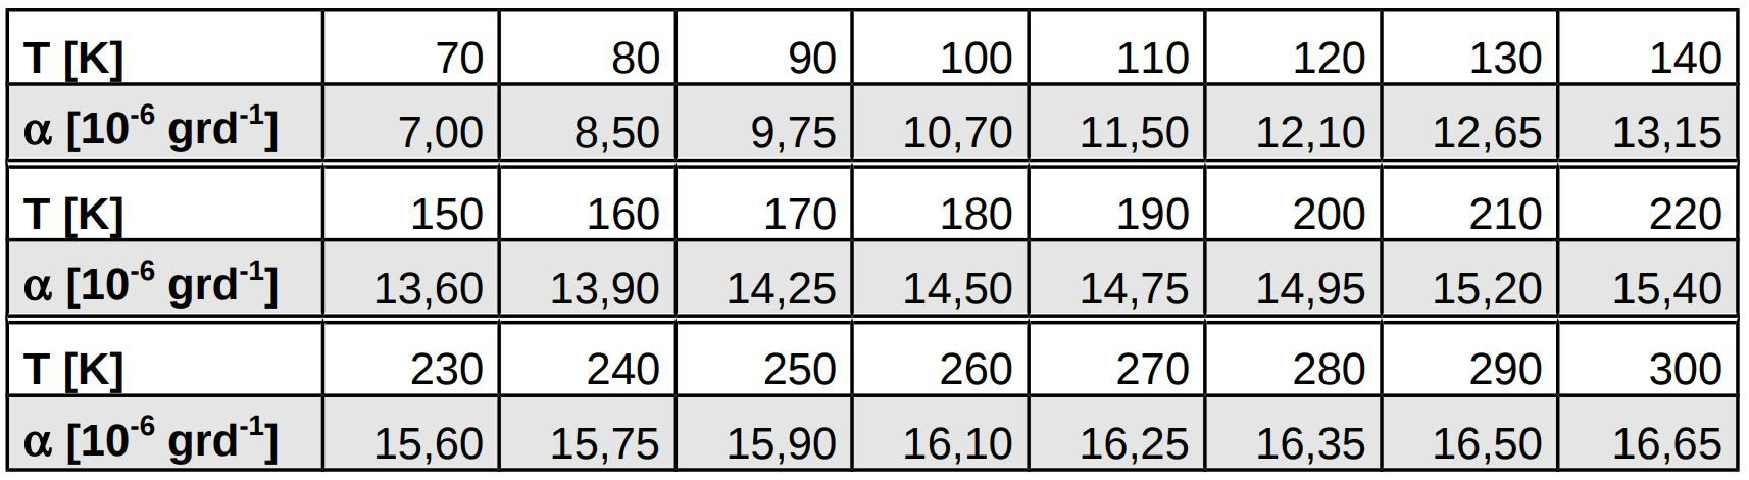
\includegraphics[scale=0.4]{alpha_table.pdf}
    \caption{Linear expansion coefficient $\alpha$ of copper as a function of the temperature \cite{V47}.}
    \label{tab:alpha}
\end{figure}
\noindent
$C\idx{V}$ is the heat capacity at a constant volume and it
can be calculated with the correction formular
\begin{equation*}
    C\idx{p}-C\idx{V} = 9 \alpha^2 \kappa V_0 T
\end{equation*}
that is depending on $C\idx{p}$, $T$, the bulk modulus $\kappa= 137 \cdot 10^9\,\unit{\pascal}$ \cite{internetchemie},
the molar volume $V_0$ and the linear expansion coefficient $\alpha$ of copper.
The molar volume is given with the density of copper $\rho= 8,96\,\unit{\frac{\gram}{\centi\meter\cubed}}$\cite{internetchemie} by 
\begin{equation*}
    V\idx{0} = \frac{M}{\rho} = 7,092 \cdot 10^{-6}\,\unit{\frac{\meter\cubed}{\mole}}.
\end{equation*}
The linear expansion coefficient is specified in the instructions for certain temperatures. But given that the measured values do not precisely 
match those provided in the given Table \ref{tab:alpha}, an approximation can be obtained by performing a linear interpolation.
According to the equation
\begin{equation*}
    \alpha(T\idx{n}) = \alpha\idx{i-1} + \frac{\alpha\idx{i}-\alpha\idx{i-1}}{T\idx{i}-T\idx{i-1}} (T\idx{n}-T\idx{i-1}),
\end{equation*}
$\alpha$ can be estimated. In Figure \ref{plot:CV} the specific heat capacity is plotted against the temperature.
\begin{figure}[h]
    \centering
    \includegraphics[scale=0.7]{build/CV_plot.pdf}
    \caption{The specific heat capacity plotted against the temperature.}
    \label{plot:CV}
\end{figure}

\newgeometry{top=1.5cm}
\input{build/table_all.tex}
\restoregeometry




\subsection{The Debye Temperatur of Copper}
In the next step the Debye temperature $\theta\idx{D}$ should be determined for the pairs of values ($C\idx{V}$,$T$).
Only the measured values up to $170\,\unit{\kelvin}$ are taken into account. Using the table in Figure \ref{tab:thetaD_per_T},
the experimental Debye temperature can be easily found.  

\begin{figure}[h]
    \centering
    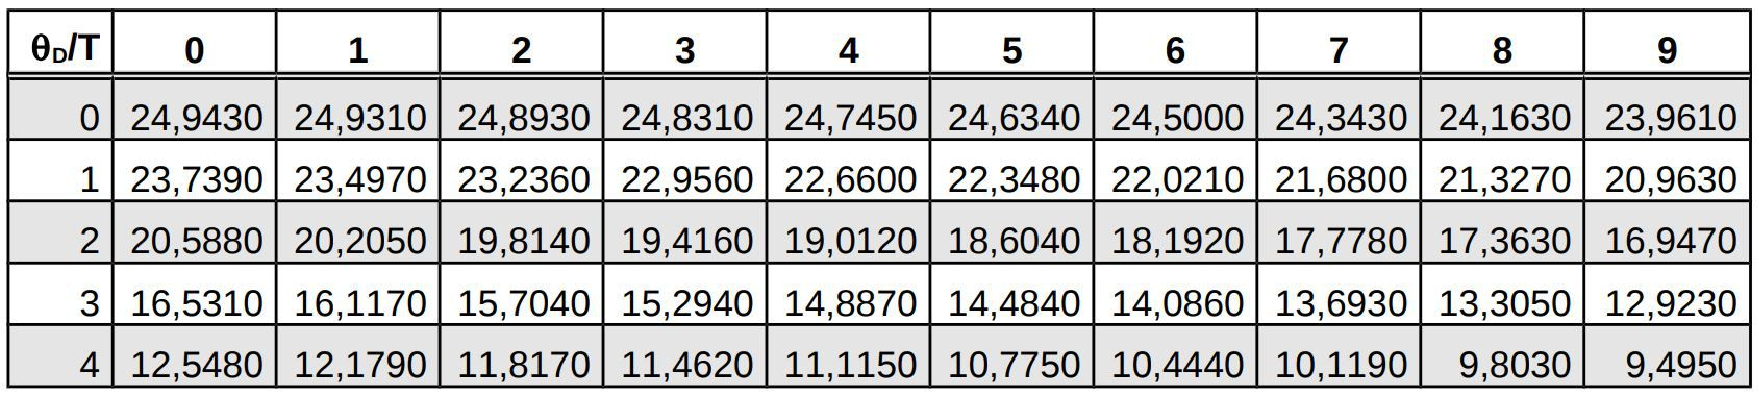
\includegraphics[scale=0.5]{thetaD_table.pdf}
    \caption{The given table to determine the Debye temperature \cite{V47}.}
    \label{tab:thetaD_per_T}
\end{figure}
\noindent
The quotient $\frac{\theta\idx{D}}{T}$ can be read by comparing the $C\idx{V}$ values with the ones in the given table. 
Then the closest value is to be selected. The left column gives the digit before the comma and the line position 
indicates the first decimal place. Thus, it can be calculated by multiplying the quotient with the respective 
temperature for which $C\idx{V}$ was calculated. Adjusted values and the Debye temperature are listed in 
Table \ref{tab:thetaD_table}. 

\input{build/table_thetaD.tex}

\noindent
Based on the equations 
\begin{equation*}
    \bar{\theta}\idx{D} = \frac{1}{N}\sum_{k = 1}^N \theta\idx{D,k}
\end{equation*}
and 
\begin{equation*}
    \Delta\bar{\theta}\idx{D} = \sqrt{\frac{1}{N(N-1)}\sum_{k = 1}^N(\theta\idx{D,k}-\bar{\theta}\idx{D})^2} \quad 
\end{equation*}
the mean and standard deviation of the Debye temperature result in 
\begin{equation*}
    \bar{\theta}\idx{D} = (347,11 \pm 55,6)\,\unit{\kelvin}.
\end{equation*}
 


\subsection{The Theoretical Debye Temperatur and Frequency}

To calculate the theoretical Debye frequency the following equation is 
required
\begin{equation*}
    \omega\idx{D}^3 = \frac{18 \pi^2 N\idx{A}}{V_0} \left (\frac{1}{v\idx{L}^3} + \frac{2}{v\idx{T}^3} \right )^{-1}.
\end{equation*}
With the Avogadro Constant $N\idx{A}= 6,022 \cdot 10^{23}\,\unit{\frac{1}{\mole}}$\cite{wiki}, 
the phase velocity of a longitudinal wave $v\idx{L}= 4,7 \cdot 10^3\,\unit{\meter\per\second}$\cite{V47}
and the phase velocity of a transversal wave $v\idx{T}= 2,26 \cdot 10^3\,\unit{\meter\per\second}$\cite{V47}
the equation gives
\begin{equation*}
    \omega\idx{D} = 4,35 \cdot 10^{13}\,\unit{\hertz}.
\end{equation*}
This allows to calculate the theoretical Debye temperature using the equation
\begin{equation*}
    \theta\idx{D}= \frac{\hbar \omega\idx{D}}{k\idx{B}}
\end{equation*}
with $\hbar= 6,63 \cdot 10^{-34}\,\unit{\joule\second}$ \cite{wiki_const} being the reduced Planck constant 
and $k\idx{B}= 1,38 \cdot 10^{-23}\,\unit{\frac{\joule}{\kelvin}}$ \cite{wiki_const} the Boltzmann constant.
This results in 
\begin{equation*}
    \theta\idx{D,th} = 332,18\,\unit{\kelvin}
\end{equation*}